\chapter{Low-Resource Data-to-Text Generation}
\label{chap:low-res}

This chapter introduces three low-resource \ac{d2t} generation approaches based on \acp{plm}. By \emph{low-resource}, we mean using as little data as possible for generating fluent and accurate texts. We develop approaches that leverage the general-domain pretraining of \acp{plm} to generate texts in domains with thousands, hundreds, or even zero training examples.

The data we focus on are \emph{\acs{rdf} triples} from factual knowledge graphs in the WebNLG dataset and \emph{key-value meaning representations} in the E2E dataset. Both datasets are described in \autoref{sec:datasets}. These datasets assume that content selection was performed beforehand, i.e., we always want to verbalize the whole input.

The most straightforward setting, presented in \autoref{sec:finetuning}, consists of finetuning mBART \cite{liuMultilingualDenoisingPretraining2020}, a pretrained transformer encoder-decoder model. For finetuning the model, we need approximately thousands of in-domain examples. We show that this baseline is powerful, achieving competitive results on a shared task for generating knowledge graph descriptions. On top of that, we show that this approach can be extended to non-English settings, namely to text generation in Russian.

In \Cref{sec:iterative,sec:pipeline}, we present approaches that can generate texts with an even more limited amount of in-domain training examples. Our key idea is to use a \ac{plm} only as a tool for improving text fluency \emph{regardless of the content} and delegating (possibly crude and basic, but factually correct) verbalization of the content to different, more controllable means. \autoref{sec:iterative} shows an approach based on a text-editing model, which has a limited vocabulary and is trained on iteratively fusing simple templates. The limited vocabulary and training objective helps the model to generate factually correct sentences. In \autoref{sec:pipeline}, we present an alternative approach that adds an ordering and aggregation step for generating more fluent texts. Moreover, we show how to train a \ac{plm} for all the steps entirely on general-domain operations, eliminating the need for in-domain training examples.

\section{Finetuning Pretrained Language Models}
\label{sec:finetuning}

\begin{refbox}
    This section is based on the paper \emph{Train Hard, Finetune Easy: Multilingual Denoising for RDF-to-Text Generation} \cite{kasnerTrainHardFinetune2020}, joint work with Ondřej Dušek, published in the Proceedings of the 3rd International Workshop on Natural Language Generation from the Semantic Web (WebNLG+) at INLG 2020.
\end{refbox}


This section introduces a simple approach for generating knowledge graph descriptions. Our approach is based on finetuning a multi-lingual \ac{plm} on linearized graphs and the accompanying human-written descriptions from the WebNLG dataset. In the WebNLG+ Shared Task, our model ranked in the first third of the leaderboard for English and the first or second for Russian on automatic metrics. It also made it in the best or second-best system cluster on human evaluation. We show that with a moderate amount of in-domain finetuning data, a simple \ac{plm}-based baseline can achieve satisfactory results in generating descriptions of knowledge graphs. We also point out its limitations, namely its inability to infer semantics of ambiguous relation labels; a topic to which we will return in \autoref{sec:rel2text}.

\subsection{WebNLG+ Shared Task}
\label{sec:webnlgp}
The WebNLG Challenge 2020\footnote{\url{https://synalp.gitlabpages.inria.fr/webnlg-challenge/challenge_2020/}} (WebNLG+; \citealp{ferreira20202020}) was the second edition of the shared task in graph-to-text generation. The task was based on the WebNLG dataset containing subgraphs from the DBpedia knowledge graph. Each subgraph is described by a set of \acs{rdf}\glsunset{rdf} triples and accompanied by crowdsourced text descriptions (see \autoref{sec:datasets}). On top of the original challenge \cite{gardentWebNLGChallengeGenerating2017}, WebNLG+ included a separate track for generating texts in Russian, in which we also participated.


\subsection{Problem Formulation}
\label{sec:mbart}
Our input is a set of \ac{rdf} triples $x \in X$, where each triple $x = (s, p, o)$ describes the relation $p$ between the entities $s$ and $o$ in the knowledge graph. Our target output $Y$ is a fluent and semantically accurate natural language description of $X$.


We formulate the task as \emph{sequence-to-sequence} generation. First, we linearize the input sequence (see \autoref{sec:neural-d2t}) in the default order using two arbitrary separator tokens: one to delimit the triple constituents and another to delimit individual triples. Using the linearized sequence as an input and the target text as an output, we finetune a pretrained encoder-decoder model for the cross-entropy objective (\autoref{eq:clm}). With the finetuned model, we generate the target texts using autoregressive decoding (see Algorithm~\ref{alg:decoding}).

% 


\subsection{Implementation}
\paragraph{Data Preprocessing} We use the provided XML WebNLG data reader\footnote{\url{https://gitlab.com/webnlg/corpus-reader}} to load and linearize the triples. For each triple, we use the \texttt{flat\_triple()} method which converts each triple into the ``\texttt{s $\vert$ p $\vert$ o}'' string, using a pipe (``$\vert$'') as a separator. We use another token not present in the training data (``$\blacktriangleright$'') for delimiting individual triples to avoid extending the model vocabulary.\footnote{We chose the separators arbitrarily, as the model is to be finetuned with the selected separators.} We linearize the triples in their default order. For the input to the model, we tokenize the data using SentencePiece tokenizer \citep{kudo2018sentencepiece} trained on the training dataset, using a vocabulary of 250,000 subword tokens.

\paragraph{Model}
We use mBART \cite{liuMultilingualDenoisingPretraining2020}, a multilingual \ac{plm} based on BART, a transformer model pretrained on text denoising (see \autoref{sec:plms}).
% In pretraining, the noise function of mBART replaces text spans of arbitrary length with a mask token (35\% of the words in each instance) and permutes the order of sentences. 
The model uses 12 layers for the encoder and 12 layers for the decoder ($\sim$680M parameters), and it is pretrained on the large-scale CC25 corpus extracted from Common Crawl, which contains data in 25 languages \citep{wenzek2020ccnet}.



\paragraph{Training} We finetune the pre-trained \texttt{mbart.CC25} model from the \textsc{fairseq} toolkit \citep{ott2019fairseq} using the default parameters,\footnote{We use dropout 0.3, attention dropout 0.1, and 1024 tokens per batch; we set the initial learning rate to 0.0003 and use polynomial decay with 2500 warmup steps. We train the model using the Adam optimizer \cite{kingma2014adam} with $\beta_1=0.9, \beta_2=0.98$ and $\varepsilon=1e-06$. For the full set of training arguments, see \url{https://github.com/facebookresearch/fairseq/tree/main/examples/mbart}.} changing only the total number of updates from 40k to 10k to reflect the smaller size of our data. We train a separate version of mBART for each language: $\text{mBART}_{\text{en}}$ on English inputs and English outputs, and $\text{mBART}_{\text{ru}}$ on English inputs and Russian outputs.



\subsection{Results}
\label{sec:finetuning:res}

\begin{table*}[t]
    \footnotesize
    \centering
    \begin{tabular}{@{}lp{12.7cm}@{}}
        \textbf{input}    & \texttt{Piotr\_Hallmann | weight | 70.308 }  $\blacktriangleright$ \texttt{ Piotr\_Hallmann | birthDate | 1987-08-25} \\
        \textbf{out (en)} & Born on August 25th 1987, Piotr Hallmann has a weight of 70.308.                                                      \\
        \midrule
        \textbf{in}       & \texttt{Ciudad\_Ayala | populationMetro | 1777539}                                                                    \\
        \textbf{out (en)} & The population metro of Ciudad Ayala is 1777539.                                                                      \\
        \midrule
        \textbf{in}       & \texttt{Bakewell\_tart | ingredient | Frangipane}                                                                     \\
        \textbf{out (ru)} & Франжипан - один из ингредиентов тарта Бейквелл.                                                                      \\[0.1cm]
        \textbf{transcr.} & Franzhipan - odin iz ingredientov tarta Bejkvell.                                                                     \\
        \textbf{transl.}  & Frangipane is one of the ingredients of the Bakewell tart.                                                            \\
    \end{tabular}
    \caption{Example outputs from the mBART model(s) finetuned for \ac{rdf}-to-text generation. (1) The model can work with unseen entities, dates, and numbers. (2) The label deviates too much from its meaning for the unseen property \texttt{populationMetro}, leading to incorrect output. (3) The model trained on Russian targets can use English data to form sentences in Russian, transcribing the entities to Cyrillic.}
    \label{tab:mbart:examples}
\end{table*}

We report on WebNLG automatic and human evaluation results, as well as our own error analysis.

\paragraph{Automatic Metrics}
The results of our approach for English are shown in \autoref{tab:mbart:results-en}. Our approach beats the baseline in all metrics and places in the first third of the submissions. While it loses performance on unseen categories, the drop is less dramatic than other competing approaches. For Russian, the results are shown in \autoref{tab:mbart:results-ru}. Our system not only beats the baseline by a large margin (as did all competing submissions), but it ranks first in 2 metrics out of 4 (BLEU, BERTScore) and second in the remaining ones.

\paragraph{Human Evaluation}

The challenge organizers ran a human evaluation campaign, asking annotators to rate the texts for data coverage, relevance, correctness, text structure, and fluency.  Each criterion has been rated with a number ranging from 0 (completely disagree) to 100 (completely agree). The scores were clustered into groups (1-5; 1 being the best), among which there are no statistically significant differences according to the Wilcoxon rank-sum test \citep{wilcoxon1992individual}.

Our systems made it into the top clusters (1 or 2) for both English and Russian. For English, our $\text{mBART}_{\text{en}}$ system ranks first for all the categories in \textit{seen domains}, and first or second in \textit{unseen entities} and \textit{unseen domains}. In total, our English system achieved rank 1 for relevance, correctness and text structure, and rank 2 for data coverage and fluency. For Russian, our $\text{mBART}_{\text{ru}}$ system ranks second for correctness and first in all other categories.


\begin{table*}[t]
    \footnotesize\centering
    \begin{tabular}{llcccccccccc}\toprule
                                     &          & \multicolumn{2}{c}{\bf BLEU} & \multicolumn{2}{c}{\bf METEOR} & \multicolumn{2}{c}{\bf ChrF++} & \multicolumn{2}{c}{\bf BERTScore} & \multicolumn{2}{c}{\bf BLEURT}                                     \\\midrule
        \multirow{2}{*}{All}         & Ours     & 50.34                        & (10)                           & 0.398                          & (8)                               & 0.666                          & (8)  & 0.951 & (8)  & 0.57 & (8)  \\
                                     & Baseline & 40.57                        & (14)                           & 0.373                          & (15)                              & 0.621                          & (15) & 0.943 & (14) & 0.47 & (12) \\\midrule
        \multirow{2}{*}{Seen Cat.}   & Ours     & 59.13                        & (10)                           & 0.422                          & (10)                              & 0.712                          & (9)  & 0.960 & (9)  & 0.58 & (14) \\
                                     & Baseline & 42.95                        & (31)                           & 0.387                          & (27)                              & 0.650                          & (28) & 0.943 & (31) & 0.41 & (31) \\\midrule
        \multirow{2}{*}{Unseen Cat.} & Ours     & 42.24                        & (10)                           & 0.375                          & (13)                              & 0.617                          & (10) & 0.943 & (11) & 0.52 & (10) \\
                                     & Baseline & 37.56                        & (12)                           & 0.357                          & (15)                              & 0.584                          & (15) & 0.940 & (12) & 0.44 & (12) \\\midrule
        \multirow{2}{*}{Unseen Ent.} & Ours     & 51.23                        & (4)                            & 0.406                          & (8)                               & 0.687                          & (7)  & 0.959 & (8)  & 0.63 & (8)  \\
                                     & Baseline & 40.22                        & (17)                           & 0.384                          & (15)                              & 0.648                          & (15) & 0.949 & (13) & 0.55 & (12) \\\bottomrule
    \end{tabular}
    \caption{Results of $\text{mBART}_{\text{en}}$ (all data, seen categories, unseen categories, unseen entities), compared to the baseline from the organizers. The numbers in brackets show the rank of each model (out of 35 submissions) with respect to the given metric.}
    \label{tab:mbart:results-en}
\end{table*}
\begin{table*}[t]
    \footnotesize\centering
    \begin{tabular}{llcccccccc}\toprule
                 & \multicolumn{2}{c}{\bf BLEU} & \multicolumn{2}{c}{\bf METEOR} & \multicolumn{2}{c}{\bf ChrF++} & \multicolumn{2}{c}{\bf BERTScore}                               \\\midrule
        Ours     & 52.93                        & (1)                            & 0.672                          & (2)                               & 0.677 & (2)  & 0.909 & (1)  \\
        Baseline & 23.53                        & (12)                           & 0.461                          & (12)                              & 0.511 & (12) & 0.836 & (12) \\\bottomrule
    \end{tabular}
    \caption{Results of $\text{mBART}_{\text{ru}}$, compared to the baseline. The numbers in brackets show the rank of each model (out of 12 submissions) if ordered by the given metric.}
    \label{tab:mbart:results-ru}
\end{table*}

\paragraph{Manual Analysis}
To better understand the nature of errors made by our system, we manually inspected a sample of 50 outputs in each language.\footnote{Automatic back-translation to English was used to facilitate understanding of Russian.} We found factual errors in 12 English outputs, mostly concentrated along the unseen categories (\emph{Scientist}, \emph{Movie}, \emph{Musical Record}). The model tends to describe musical works and movies in terms of written works (``written'', ``published'' etc.), i.e., the closest seen category. There are also several swaps in roles of the entities (e.g., ``is to southeast'' instead of ``has to its southeast'', ``follows'' instead of ``is followed by'' etc.).

In a few cases, the model hallucinates a relation not specified in the data (e.g., ``born on January 1, 1934 in Istanbul'' when a date of birth and current residence is given, not the birthplace) or is not able to infer background knowledge not given on the input (it talks about a dead person in the present tense).
% The swaps in roles and hallucinated relations also occured in Russian; in addition, we found a hallucinated (correct) airport name and a few forgotten ingredients for a dish from a long list. 
Factual errors in Russian were less frequent (9 sentences), which is expected as there are no unseen categories. Moreover, the system shows an impressive performance at translating entity names from the English \ac{rdf} into Russian.

We further found 10 outputs with suboptimal phrasing in English and 9 in Russian, where the model did not connect properties of the same type in a coordination (e.g., two musical genres for a record) or gave numbers without proper  units (e.g., ``runtime of 89.0'' or ``area of 250493000000.0'').

\subsection{Discussion}
\paragraph{Why does our approach work?} Our solution benefits from the pretrained mBART model, which has absorbed vast amounts of factual world knowledge \cite{petroni2019language}. Combined with its ability of producing fluent texts, the model naturally performs well at generating short, factually-grounded sentences. Moreover, multilingual pretraining of the model allows us to use a single architecture for both English and Russian. As other solutions in the challenge also used pretrained models with similar architecture (but not consistently even performance), we should emphasize the need for a careful choice of hyperparameters.\footnote{Nevertheless, in our case, we achieved satisfactory results without departing from the default setup.}

\paragraph{Where are its limitations?} Our approach is data-driven, and thus it depends on the access to the high-quality training set of in-domain data. Such data is generally not readily available for other domains, and gathering it requires substantial human effort and financial resources. The generalization to other languages also does not come cheap: English and Russian are the two most represented languages in the mBART pre-training corpora (ca. 300 GB of data each) and we can expect the performance of our model to be lower with low-resource languages.

There are also limitations related to the formulation of the task itself. As we noted in \autoref{sec:finetuning:res}, the performance of our model is noticeably lower on categories unseen in training.  We show later in \autoref{sec:rel2text}, that this issue is hard to circumvent: the best solution is to leverage the model's language understanding by using human-readable labels. The size of the input examples is also somehow limited (no more than seven triples); therefore, we cannot expect the model to perform equally well for inputs of arbitrary size.
% That being said, the current setup may still cover practical scenarios with pre-selected content.

\paragraph{What are the ways forward?} The 2023 WebNLG Shared Task featured our system as the baseline for the track for graph-to-text generation in Russian \cite{cripwell2023WebNLGShared2023}. The organizers of the task note that \textit{``results on Russian for the present edition provide very small improvements over the best results for 2020.''} These results suggest that (1) the WebNLG task is saturated, yielding only very small improvements regardless of the technique (at least for high-resource languages), and (2) fixing the long tail requires different, more principled approaches allowing to identify and correct unclear input cases (e.g., by human interventions based on model uncertainty). However, these interventions may yield only small improvements on automatic metrics and may not be possible in the framework of the shared task.


In \Cref{sec:iterative,sec:pipeline}, we introduce approaches for \ac{d2t} generation which cut down on the need for extensive amount of in-domain training data. These approaches still rely on the existence of \acp{plm}, but they are given inductive bias necessary for the task at hand: namely, that the goal is to transform a disfluent input (i.e., the structured data in its original format) into a fluent output (i.e., the structured data expressed in natural language). These approaches make it possible to build data-driven approaches for \ac{d2t} generation for domains lacking high-quality training data.

% There may be some limitation related to factual knowledge: the model may be prone to generating factually correct sentences \emph{regardless} of the input.


\paragraph{What about large language models?} Suprisingly, our findings are still valid in the era of \acp{llm}. We recommend the works of \citet{axelssonUsingLargeLanguage2023} and \citet{yuanEvaluatingGenerativeModels2023} for elucidating this topic. As shown in these works, the GPT-3.5 model \cite{chatgpt} \emph{does not} generally outperform finetuned systems on the WebNLG dataset. In particular, \citet{axelssonUsingLargeLanguage2023} compared zero-shot performance GPT-3.5 to the systems of WebNLG 2020 challenge and found the model achieves similar performance as our system on English, while not outperforming the best systems in the challenge. The model also still makes semantic errors (as we also discuss in \autoref{sec:quintd}) and performs significantly worse on Russian data than on English data. As shown in \citet{yuanEvaluatingGenerativeModels2023}, the model may be be hard to control with respect to the output format. It should be also noted that GPT-3.5 is given unfair advantage during evaluation, as it may have memorized the outputs on the WebNLG test set \cite{balloccu2024leak}.



\section{Iterative Sentence Fusion}
\label{sec:iterative}

\begin{refbox}
    This section is based on the paper \emph{Data-to-Text Generation with Iterative Text Editing} \cite{kasnerDatatoTextGenerationIterative2020}, joint work with Ondřej Dušek, published in the Proceedings of the 13th International Conference on Natural Language Generation (INLG 2020).
\end{refbox}

In this section, we present an approach for generating semantically accurate texts from structured data in low-resource settings. Our approach builds on a text-editing model trained on the task of \emph{sentence fusion}. After transforming individual data items to text using trivial templates, we iteratively improve the resulting text by applying sentence fusion, filtering, and re-ranking.  Although our approach gets lower scores on lexical similarity metrics on WebNLG and E2E datasets than the state-of-the-art approaches, it achieves high levels of semantic accuracy due to the limited scope of the sentence fusion model and the guaranteed presence of the entities. We also demonstrate that our task formulation allows zero-shot \ac{d2t} generation by training a model on a general-domain dataset for sentence fusion. The code for the experiments is available on Github.\footnote{\url{https://github.com/kasnerz/d2t_iterative_editing}}


\subsection{Motivation}
\label{sec:text-editing}
We aim to improve the semantic accuracy \ac{d2t} generation. Other works have pursued this goal, e.g., by adapting the decoding algorithm \cite{tianStickingFactsConfident2020}, improving the robustness of the model by injecting noise in its hidden states \cite{kedzie_good_2019}, or self-training with a natural language understanding model \cite{nieSimpleRecipeReducing2019}. Our approach is inspired by the systems which use a \emph{generate-then-rerank} approach \citep{dusekSequencetoSequenceGenerationSpoken2016,juraska_deep_2018}, e.g., using a classifier to filter incorrect outputs \cite{harkousHaveYourText2020}.

To generate outputs with sufficient semantic accuracy for the filtering step, we take advantage of three facts: (1) we can lexicalize individual data items using trivial templates, (2) concatenating the lexicalizations tends to produce an unnatural sounding but semantically accurate output, and (3) a \ac{plm} trained on improving the output fluency can be used for combining the lexicalizations.

% \textsc{LaserTagger} \cite{malmi2019lasertagger}, which we use in our approach, is a sequence tagging model based on the transformer architecture with BERT \cite{devlinBERTPretrainingDeep2019} as the encoder backbone. Other recent text-editing models without a pre-trained backbone include EditNTS \citep{dong} and Levenshtein Transformer \citep{gu2019levenshtein}.

% Concurrently with our work, \citet{kale2020few} explored using templates for dialogue response generation. %\ODdel{Unlike our work,} 
% They use the sequence-to-sequence T5 model \citep{raffel2019exploring} to generate the output text from scratch instead of iteratively editing the intermediate outputs, which leaves less control over the model.


\subsection{Method}
\label{sec:text-editing-exp}
We focus on data structured as \ac{rdf} triples. In our approach, we start from single-triple templates and iteratively fuse them into the resulting text while filtering and reranking the results. We first detail the main components of our system (template extraction, sentence fusion, \ac{plm} scoring) and then give the overall description of the generation algorithm.

\begin{figure*}[t]
    \centering
    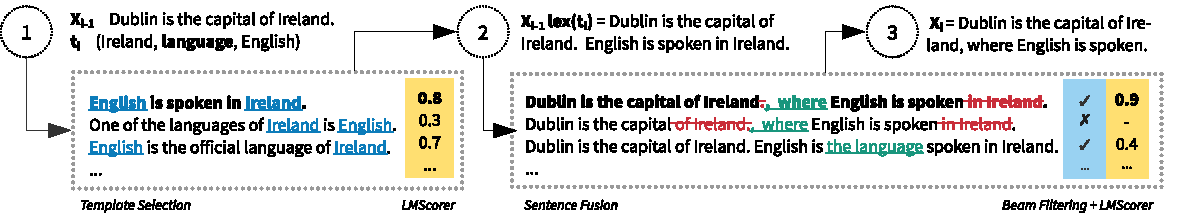
\includegraphics[width=\textwidth]{img/d2t_text_editing}
    \caption{A single iteration of our algorithm for iterative \ac{d2t} generation. In Step 1, the template for the triple is selected and filled. In Step 2, the sentence is fused with the template. In Step 3, the result for the next iteration is selected from the beam by filtering and language model scoring.}\label{fig:iterative:alg}
\end{figure*}



\paragraph{Template Extraction}
We collect a set of templates for each unique predicate. We use two approaches: (a) handcrafting the template manually for each predicate in the training set and (b) automatically extracting the template from the lexicalizations of the examples in the training set. For unseen predicates, we add a single fallback template: \textit{The <predicate> of <subject> is <object>.}


\paragraph{Sentence Fusion}
We train a model for the task of \emph{sentence fusion}, i.e., combining sentences into a coherent text \cite{barzilay2005sentence}.
%We train an independent in-domain sentence fusion model for each dataset. 
To construct the training data for the model, we select pairs of examples $(X, X')$ and their corresponding text descriptions $(Y, Y')$ from the original training set such that the examples consist of $(k, k+1)$ triples and have $k$ triples in common. This leaves us with an extra triple $x_{k+1}$ present only in $X'$. For each training example, we use the concatenated sequence $Y \mathrm{lex}(x_{k+1})$ as a source and the sequence $Y'$ as a target, where $\mathrm{lex}(x_{k+1})$ denotes lexicalizing the triple $x_{k+1}$ using an appropriate template.
As a result, the model learns to integrate $Y$ and $x_{k+1}$ into a single coherent expression.


\paragraph{PLM Scoring} For re-ranking the text, we use an additional component for computing text fluency, which we refer to as \textsc{LMScorer}.
As described in \autoref{sec:evaluation}, we use perplexity of the text under a a \ac{plm}, computing the score of the output text $Y$ composed of tokens $(y_1, \ldots, y_n)$ as a geometric mean of the token conditional probability:
\begin{align}
    \operatorname{score}(Y) = \Bigg( \prod_{i=1}^{n}{P(y_i|y_1, \ldots, y_{i-1})} \Bigg)^{\frac{1}{n}}.
\end{align}




\paragraph{Generation Algorithm}
The input of the algorithm (\autoref{fig:iterative:alg}) is a set of $T$ ordered triples. First, we lexicalize the triple $x_0$ to get the output text $Y_0$ by filling the available templates and using the template with the best score from \textsc{LMScorer}.
% This promotes templates which sound more natural for particular values.
In each of the following steps $i=(1, \ldots, T-1)$, we lexicalize the triple $x_i$ and concatenate it with $Y_{i-1}$.  To improve the fluency of the text, we use the sentence fusion model with beam search to produce $k$ hypotheses. We filter and re-rank the hypotheses (see the next paragraph), getting $Y_{i}$ for the next step. The output is the text $Y_{T-1}$ from the final step.


\paragraph{Filtering and Re-ranking} In each decoding step, we remove hypotheses in the beam missing any entity from the input data using a simple heuristic based on string matching. We rescore the remaining hypotheses in the beam with \textsc{LMScorer} and set the hypothesis with the best score as $Y_{i}$. In case there are no sentences left in the beam after the filtering step, we let $Y_{i}$ be the text in which the lexicalized $x_i$ is appended after $Y_{i-1}$ without sentence fusion, ensuring the semantic accuracy of the text.

%For the E2E dataset, we first try to find a pair of predicates for which there is a template extracted from the data, and only use the handcrafted templates for the single predicates in the subsequent steps. 
%The final beam filtering step is a simple heuristic, checking if all entities from the input triples are present in the output.


\subsection{Implementation}
\label{sec:iterative:implementation}

\begin{table}[t]
    \centering\footnotesize
    \begin{tabular}{@{}lllll@{}}
        \textbf{dataset} & \textbf{method} & \textbf{predicate}          & \textbf{example \#1}                       & \textbf{example \#2}                \\\midrule
        WebNLG           & extracted       & \texttt{foundedBy}          & \et{} was the founder of \eh{}.            & \eh{} was founded by \et{}.         \\
        E2E              & extracted       & \texttt{area}+\texttt{food} & \eh{} offers $\ets$ cuisine in the $\etf$. & \eh{} in $\etf$ serves $\ets$ food. \\
        E2E              & manual          & \texttt{near}               & \eh{} is located near \et{}.               & \et{} is close to \eh{}.
    \end{tabular}
    \caption{Examples of templates we used in our experiments. The markers \eh{} and \et{} are placeholders for the subject and the object, respectively. The templates for the single predicates in the WebNLG dataset and the pairs of predicates in the E2E dataset are extracted automatically from the training data; the templates for the single predicates in E2E are created manually.}
    \label{tab:iterative:templates_ex}
\end{table}


\paragraph{Template Extraction} We experiment with the WebNLG and E2E datasets (see \autoref{sec:datasets}). For WebNLG, we extract the templates from the training examples containing only a \textit{single} triple. In the E2E dataset, there are no such examples; therefore, we first extract the templates for \textit{pairs} of predicates, using them as a starting point for the algorithm to leverage the lexical variability in the data (manually filtering out the templates with semantic noise). We also create a small set of templates for each \textit{single} predicate manually, using them in the subsequent steps of the algorithm.\footnote{In the E2E dataset, the data is in the form of key-value pairs. We transform the data to \ac{rdf} triples by using the name of the restaurant as a \textit{subject} and the rest of the pairs as \textit{predicate} and \textit{object}. This creates \textit{n-1} triples for \textit{n} pairs.} See \autoref{tab:iterative:templates_ex} for examples of templates we used in our experiments.

\paragraph{Sentence Fusion Model} We base our sentence fusion model on the text-editing model \textsc{LaserTagger} \cite{malmi2019lasertagger}. \textsc{LaserTagger} generates outputs by tagging inputs with edit operations (\texttt{KEEP} a token, \texttt{DELETE} a token, and \texttt{ADD} a phrase before the token), which makes it suitable for tasks where the output highly overlaps with the input. An important feature of \textsc{LaserTagger} is its limited vocabulary size, consisting of $k$ most frequent (possibly multi-token) phrases used to transform inputs to outputs in the training data. After the vocabulary is precomputed, all infeasible examples in the training data are filtered out. At the cost of limiting the number of training examples, this filtering makes the training data cleaner by removing outliers. The limited vocabulary also makes the model less prone to hallucination errors.

\paragraph{LMScorer} As the \textsc{LMScorer} backend, we use the pre-trained GPT-2 language model \citep{radford2019language} from the Transformers repository\footnote{\url{https://github.com/huggingface/transformers}} \citep{wolf2019HuggingFacesTS}. We compute the perplexity scores using the \textit{lm-scorer}\footnote{\url{https://github.com/simonepri/lm-scorer}} package.








\subsection{Experiments}
\paragraph{Base Experiments} As a \emph{baseline}, we generate the best templates according to \textsc{LMScorer} without applying the sentence fusion (i.e., always using the fallback). For the \emph{sentence fusion} experiments, we use \textsc{LaserTagger} with the autoregressive decoder with a beam of size 10. We use all reference lexicalizations and the vocabulary size $V=100$, following our preliminary experiments. We finetune the model for 10,000 updates with batch size 32 and learning rate $2 \times 10^{-5}$.
For the beam filtering heuristic, we check for the presence of entities by simple string matching in WebNLG; for the E2E dataset, we use a set of regular expressions from \citet{dusekSemanticNoiseMatters2019}. We process the triples in their default order.

\paragraph{Zero-shot Generation} Additionally, we conduct a \textit{zero-shot} experiment. We train the sentence fusion model with the same setup, but instead of the in-domain datasets, we use a subset of the \emph{balanced-Wikipedia} portion of the \textsc{DiscoFuse} dataset \cite{geva-etal-2019-discofuse}. In particular, we use the discourse types frequently occurring in our datasets, filtering the discourse types irrelevant to our use case.


% \vspace{-3mm}
\subsection{Results}


\begin{table*}[t]% \begin{adjustbox}{max width=\textwidth}
    \centering\footnotesize
    \begin{tabular}{lcccc<{\hspace{2mm}}c>{\hspace{2mm}}cccc} \toprule
                         & \multicolumn{4}{c}{\bf WebNLG} &            & \multicolumn{4}{c}{\bf E2E}                                                                                                                                                                          \\
        \cmidrule{2-5} \cmidrule{7-10}
                         & {\it BLEU}                     & {\it NIST} & \hspace{-1mm}{\it METEOR}\hspace{-1mm} & \hspace{-1mm}{\it ROUGE$_L$}\hspace{-1mm} &  & {\it BLEU} & {\it NIST} & \hspace{-1mm}{\it METEOR}\hspace{-1mm} & \hspace{-1mm}{\it ROUGE$_L$}\hspace{-1mm} \\
        {\bf baseline}   & 0.277                          & 6.328      & 0.379                                  & 0.524                                     &  & 0.207      & 3.679      & 0.334                                  & 0.401                                     \\
        {\bf zero-shot } & 0.288                          & 6.677      & 0.385                                  & 0.530                                     &  & 0.220      & 3.941      & 0.340                                  & 0.408                                     \\
        {\bf w/fusion }  & 0.353                          & 7.923      & 0.386                                  & 0.555                                     &  & 0.252      & 4.460      & 0.338                                  & 0.436                                     \\
        {\bf SFC }       & 0.524                          & -          & 0.424                                  & 0.660                                     &  & 0.436      & -          & 0.390                                  & 0.575                                     \\
        {\bf T5 }        & 0.571                          & -          & 0.440                                  & -                                         &  & -          & -          & -                                      & -                                         \\ \bottomrule
    \end{tabular}
    \caption{Results of automatic metrics on the WebNLG and E2E test sets.}
    \label{tab:results}
    % \end{adjustbox}
\end{table*}
\paragraph{Accuracy vs.\ Fluency}
On lexical similarity metrics (\autoref{tab:iterative:output}), our system lags behind the state-of-the-art approaches selected for comparison: the Semantic Fidelity Classifier (SFC; \citealp{harkousHaveYourText2020}) and the finetuned T5 model (T5; \citealp{kaleTexttoTextPreTrainingDatatoText2020}). However, both the fusion and the zero-shot approaches show improvements over the baseline. It is also important to note that our approach ensures zero entity errors: the entities are filled verbatim into the templates, and if an entity is missing in the whole beam, a fallback is used instead (although semantic inconsistencies can still occur, e.g., if a verb or function words are missing).

\paragraph{Error Analysis} The fused sentences in the E2E dataset, where all the objects are related to a single subject, often lean towards compact forms, e.g., \textit{Aromi is a family friendly chinese coffee shop with a low customer rating in riverside}. On the contrary, the sentence structure in WebNLG mostly follows the structure from the templates, and the model makes minimal changes to fuse the sentences. See \autoref{tab:iterative:output} an example of the system output. Of all steps, 28\% are fallbacks (no fusion is performed) in WebNLG and 54\% in the E2E dataset.
The higher number of fallbacks in the E2E dataset can be explained by a higher lexical variability of the references, together with a higher number of data items per example. This variability makes it harder for the model to maintain the text coherency over multiple steps.


\begin{table*}[t] \footnotesize
    \begin{tabular}{l p{12cm}}
        \textbf{Triples}   & \textit{(Albert Jennings Fountain, deathPlace, New Mexico Territory); (Albert Jennings Fountain, birthPlace, New York City); (Albert Jennings Fountain, birthPlace, Staten Island)} \\ \midrule
        \textbf{Step \#0}  & Albert Jennings Fountain died in New Mexico Territory.                                                                                                                              \\
        \textbf{Step \#1}  & Albert Jennings Fountain, who died in New Mexico Territory, was born in \greenund{New York City}.                                                                                   \\
        \textbf{Step \#2}  & Albert Jennings Fountain, who died in New Mexico Territory, was born in New York City, \greenund{Staten Island}.                                                                    \\ \midrule
        \textbf{Reference} & Albert Jennings Fountain was born in Staten Island, New York City and died in the New Mexico Territory.
    \end{tabular}
    \caption{An example of correct behavior of the algorithm on the WebNLG dataset. Newly added entities are underlined, the output from Step \#2 is the output text.}\label{tab:iterative:output}
\end{table*}

\paragraph{Templates} On average, there are 12.4 templates per predicate in WebNLG and 8.3 in the E2E dataset. In cases where the set of templates is more diverse, e.g., if the template for the predicate \textit{country} has to be selected from \{\textit{<subject> is situated within <object>, <subject> is a dish found in <object>}\}, \textsc{LMScorer} helps to select the semantically accurate template for the specific entities. The literal copying of entities can be too rigid in some cases, e.g., \textit{Atatürk Monument (İzmir) is made of ``Bronze''}.

\paragraph{Zero-shot Experiments} The zero-shot model trained on \textsc{DiscoFuse} is able to correctly pronominalize or delete repeated entities and join the sentences with conjunctives, e.g.\ \textit{William Anders was born in British Hong Kong\underline{, and was} a member of the crew of Apollo 8}. While the model makes only a limited use of sentence fusion, it makes the output more fluent while keeping strong guarantees of the output accuracy.





\subsection{Discussion}

% \textsc{LaserTagger} does not allow arbitrary reordering of words in the sentence, which can limit the expressiveness of the sentence fusion model. Consider the example in \autoref{fig:iterative:alg}: in order to create a sentence \textit{English is spoken in Dublin, the capital of Ireland}, the model has to delete and re-insert at least one of the entities, e.g., \textit{English}, which has to be present in the vocabulary.

% Building a high-quality sentence fusion model, which lies at the core of our approach, remains a challenge \cite{lebanoff2020learning}. Our simple extractive approach relying on existing D2T datasets may not produce sufficient amount of clean data. On the other hand, the phenomena covered in the \textsc{DiscoFuse} dataset are too narrow for the fully general sentence fusion. We believe that training the sentence fusion model on a larger and more diverse sentence fusion dataset, built e.g. in an unsupervised fashion \cite{lebanoff-etal-2019-scoring}, is a way to improve the robustness of our approach.

% Fluency of the output sentences may be also improved by allowing more flexibility for the order of entities, either by including an ordering step in the pipeline \citep{moryossef2019astep}, or by using a text-editing model that is capable of explicit reordering of words in the sentence \cite{mallinson2020felix}. Splitting the data into smaller batches (i.e. setting an upper bound for the number of sentences fused together) could also help to improve the consistency of results with a higher number of data items.

% Our string matching heuristic is quite crude and may lead to a high number of fallbacks. Introducing a more precise heuristic, such as a semantic fidelity classifier \citep{harkous2020have}, or a model trained for natural language inference \citep{dusek2020nli} could help to promote lexical variability of the text.

% Finally, we note that the text-editing paradigm allows to visualize the changes made by the model, introducing the option to accept or reject the changes at each step, and even build a set of custom rules on top of the individual edit operations based on the affected tokens. This flexibility could be useful for tweaking the model manually for a production system.


% \subsection{Conclusions}
% We proposed a simple and intuitive approach for D2T generation, splitting the process into two steps: lexicalization of data and improving the text fluency. A trivial lexicalization helps to promote fidelity and domain independence while delegating the subtle work with language to neural models allows to benefit from the power of general-domain pre-training. While a straightforward application of this approach on the WebNLG and E2E datasets does not produce state-of-the-art results in terms of automatic metrics, the results still show considerable improvements above the baseline. We provided insights into the behavior of the model, highlighted its potential benefits, and proposed the directions for further improvements.


\section{Pipeline of Text-to-Text Neural Modules}
\label{sec:pipeline}
\begin{refbox}
    This section is based on the paper \emph{Neural Pipeline for Zero-Shot Data-to-Text Generation} \cite{kasner2022neural}, joint work with Ondřej Dušek, published in the Proceedings of the 60th Annual Meeting of the Association for Computational Linguistics (ACL 2022).
\end{refbox}

In this section, we further develop the approach from \autoref{sec:iterative} for generating semantically accurate text from structured data. The main limitation of the previous approach, based on iterative transformations of simple templates, was the limited fluency of the output texts. To improve text fluency, we propose adding modules for ordering and aggregation, making the process a three-step pipeline. We also propose a way to make each of these steps trainable on a generic synthetic corpus. We confirm that on WebNLG and E2E datasets, our approach can get lower rates of omissions and hallucinations than prior approaches according to a semantic accuracy metric while achieving levels of lexical similarity comparable to some of the prior systems; all of this without the need for in-domain training data. Our code and data is available on Github.\footnote{\url{https://github.com/kasnerz/zeroshot-d2t-pipeline}}


\subsection{Motivation}
Our experiments in \autoref{sec:iterative} with iterative sentence fusion led to several observations:

\begin{enumerate}
    \item The fixed order of triples limits the expressivity of the model, leading to unnatural outputs.
    \item Using the sentence fusion model on every sentence boundary tends to produce sentences which are too compact.
    \item Text-editing models underperform state-of-the-art autoregressive models in terms of output quality.
\end{enumerate}

Following these observations, we improve our approach by (1) inserting a triple-ordering step in the process, (2) replacing the sentence fusion with paragraph compression, and (3) basing the approach on trainable autoregressive models.


Our approach follows the idea of pipeline-based approaches (see \autoref{sec:d2t-pipeline}). In particular, our pipeline follows the concept of pipelines based on iterative improvements of simple templates  \cite{laha2020scalable} and neural modules \cite{ferreiraNeuralDatatotextGeneration2019}. We focus on the \emph{ordering} and \emph{aggregation} steps, which were shown to improve the quality of \ac{d2t} generation outputs in domain-specific setups \cite{moryossef2019improving,moryossef2019step,trisedyaSentenceGenerationEntity2020,su2021plan}.

In contrast to previous approaches, our pipeline is fully trainable on general-domain data, i.e., without using any training data from target \ac{d2t} datasets. By eliminating the need for human references, we get rid of the costly and time-consuming data collection process. At the same time, we also avoid the brittleness of few-shot approaches, which are sensitive to the choice of finetuning examples \cite{chenFewShotNLGPreTrained2019,suFewShotTabletoTextGeneration2021,changSelectGenChallengeFinding2021}.

\subsection{Method}
\label{sec:pipeline:method}
\begin{figure}[t]
    \centering
    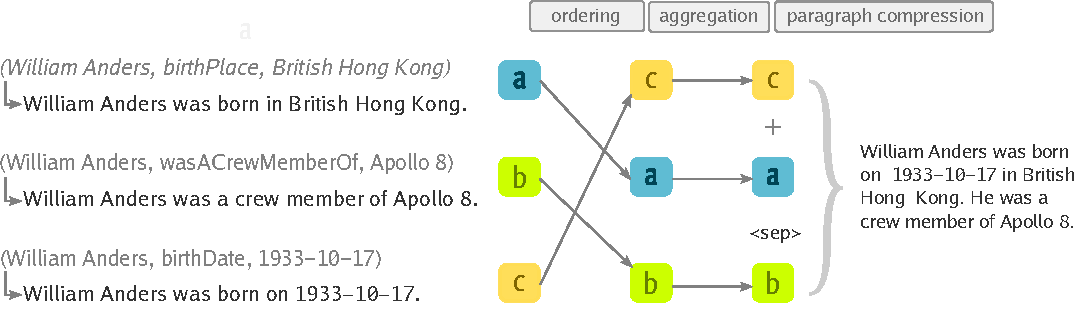
\includegraphics[width=\textwidth]{img/zeroshot_pipeline.pdf}
    \caption{A scheme of our approach for zero-shot data-to-text generation from RDF triples. After a simple transformation of triples to facts, we apply the pipeline of modules for (1) ordering, (2) aggregation, (3) paragraph compression. Individual modules are trained on a large general-domain text corpus and operate over text in natural language.}\label{fig:zeroshot:pipeline}
\end{figure}
Here, we provide a formal description of our approach. Similarly to \Cref{sec:finetuning,sec:iterative}, we focus on the task of producing a natural language description $Y$ a set of \ac{rdf} triples $x \in X$, where each triple $x = (s, p, o)$ describes the relation $p$ between the entities $s$ and $o$ in the knowledge graph.

Given a set of triples $X$ on the input, we:
\begin{enumerate}
    \item transform the triples into \textit{facts}, i.e., short sentences in natural language,
    \item sort the facts using an \textit{ordering} module,
    \item insert sentence delimiters between the ordered facts using an \textit{aggregation} module,
    \item input the ordered sequence of facts with delimiters into a \textit{paragraph compression} module, which generates the final description $Y$.
\end{enumerate}

\paragraph{Transforming Triples to Facts}

The first step in our pipeline involves transforming each of the input triples $x \in X$ into a fact $f \in F$  using a transformation $T: X \rightarrow F$. We define a fact $f$ as a single sentence in natural language describing $x$.
The transformation serves two purposes: (a) preparing the data for the subsequent text-to-text operations and (b) introducing in-domain knowledge about the semantics of individual predicates.


% This step can be realized e.g. using a simple template for each predicate (cf. §\ref{sec:templates_model}).
% Several neural methods for this task were proposed, using either interactions between pairs of sentences \cite{chen2016neural,li2017neural}, global interactions \cite{gong2016end,wang2019hierarchical}, or combination of both \cite{cui2020bert}. We base our ordering module (§\ref{sec:ord_model}) on the recent work of \citet{calizzano2021ordering}, who use a pointer network \cite{wang2019hierarchical,vinyals2015pointer} on top of a PLM.


\paragraph{Ordering} We assume that the default order of triples $X$ is random. Note, however, that $F$ is a set of meaningful sentences. We can use this to our advantage and apply a sentence ordering module \cite{barzilay2001sentence,lapata2003probabilistic} to maximize the coherency of the paragraph resulting from their concatenation. The sentence ordering module $O(F)$ produces an ordered sequence of facts: $F_o = \{f_{o_1}, \ldots, f_{o_n}\}$, where $o_{1:n}$ is a permutation of fact indices. An example outcome of such operation may be grouping together facts mentioning \textit{birth date} and \textit{birth place} of a person, followed by their \textit{occupation}, as it is shown in \autoref{fig:zeroshot:pipeline}. The ordering module allows downstream modules to focus only on operations over neighboring sentences.


\paragraph{Aggregation} Some facts will be typically mentioned together in a single sentence. Considering the previous example, \textit{occupation} is likely to be mentioned separately, while \textit{birth date} and \textit{birth place} are likely to be mentioned together. We make these decisions using the aggregation module, which takes a sequence of ordered facts $F_o$ as input and produces a sequence of sentence delimiters $A(F_o) = \{\delta_{o_1}, \delta_{o_2}, \ldots, \delta_{o_{n-1}}\}$; $\delta_{i} \in \{0, 1\}$.
% The output $\delta_{i}=1$ means that the neighboring facts should be mentioned separately, i.e. the neighboring sentences should \textit{not} be fused. Conversely, 
Unlike previous works \cite{wiseman2018learning,shao-etal-2019-long,shen-etal-2020-neural,xuAGGGENOrderingAggregating2021}, which capture the segments corresponding to individual parts of the input as latent variables, we simply insert delimiters into the ordered sequence of facts to mark sentence boundaries. The output $\delta_{i}=0$ means that the facts should be aggregated, and their corresponding sentences should be fused. Note that the markers serve only as a hint for the paragraph compression module, i.e., the sentences are not fused in this step.



\paragraph{Paragraph Compression}  The \ac{pc} module takes as input the ordered sequence of facts with delimiters $F_a = \{f_{o_1}, \delta_{o_1}, f_{o_2}, \ldots, \delta_{o_{n-1}}, f_{o_n}\}$ and produces the final text $Y$.  It has two main objectives: (a) \textit{fusing} related sentences, i.e., sentences $i$ and $j$ in between which $\delta_{i}=0$, and (b) \textit{rephrasing} the text to improve its fluency, e.g., fixing disfluencies in the templates or replacing noun phrases with referring expressions. Unlike in text summarization or sentence simplification, the edits will typically be minor since we aim to preserve the semantics of the text.



\subsection{\textsc{WikiFluent} Corpus}
\label{sec:pipeline:wikifluent}
For training the modules, we need to build a corpus in which (1) the input is a set of simple, template-like sentences, (2) the output is a fluent text in natural language preserving the semantics of the input. Here, we propose a way how to build such a large-scale synthetic corpus from English Wikipedia. Our resulting corpus (\textsc{WikiFluent}) is orders of magnitude larger than the in-domain \ac{d2t} datasets and provides training data for all the modules in our pipeline.

% we collect a large-scale synthetic corpus \textsc{WikiFluent}. Our goal is to build a corpus covering a broad range of domains and capturing the sentence style in D2T generation. In other words, we . As we describe below in detail, we achieve that by using human-written paragraphs in English Wikipedia and applying \textit{split-and-rephrase} and  \textit{coreference resolution} models to obtain synthetic source texts. The process is illustrated in Figure \ref{fig:wikifluent}; corpus statistics are included in Appendix \ref{app:stats}.

\paragraph{Data Source} For building the \textsc{WikiFluent} corpus, we first extracted 934k first paragraphs of articles from a Wikipedia dump\footnote{\texttt{enwiki-20210401-pages-articles-multistream}} using WikiExtractor \cite{Wikiextractor2015}. Wikipedia is commonly used for large-scale pretraining of D2T generation models, as it provides a source of neutral texts based on factual data \cite{jinGenWikiDatasetMillion2020,chenKGPTKnowledgeGroundedPreTraining2020}.
% Although it is not bias-free, it provides more balanced sample of natural language use than typical D2T generation datasets. 
We used the first paragraphs of Wikipedia entries with lengths between 30-430 characters, filtering out lists, disambiguations, and malformed paragraphs. To balance the lengths of inputs, we divided the paragraphs according to their length into four equally-sized bins (30-130 characters, etc.) and selected 250k examples from each bin.



\begin{figure}[t]
    \centering
    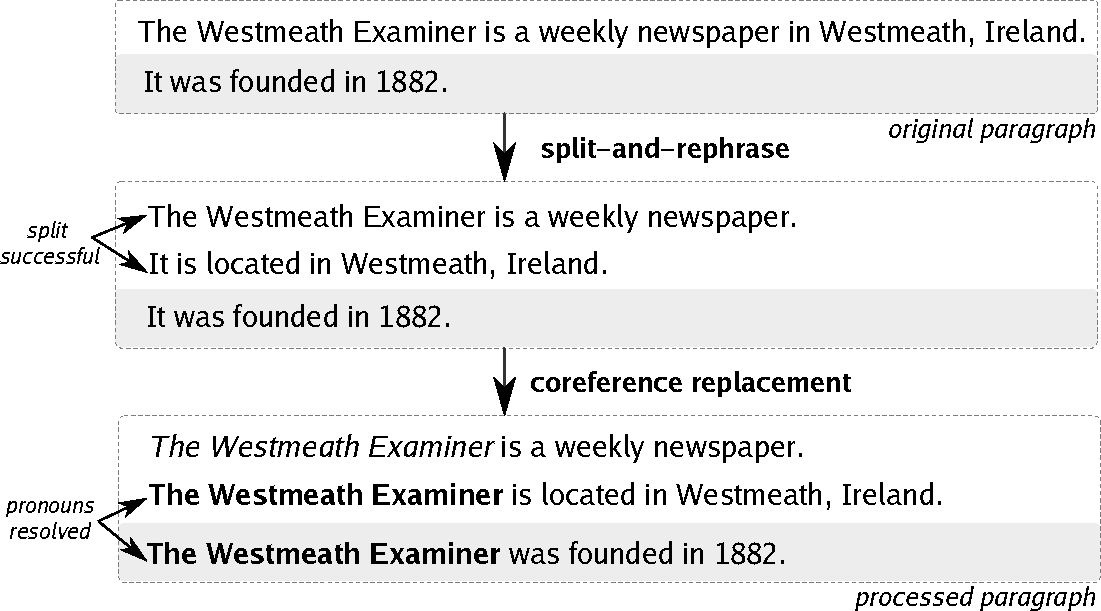
\includegraphics[width=0.7\textwidth]{img/wikifluent.pdf}
    \caption{The building process of the \textsc{WikiFluent} corpus. We apply a split-and-rephrase model on each sentence in the paragraph and resolve coreferences in the split sentences. The result is a set of simple sentences that convey the same meaning as the original paragraph. The synthesized sentences are used as \textit{input} in our models; the original human-written texts are used as \textit{ground truth}.}\label{fig:wikifluent}
\end{figure}

\begin{table*}[t]
    \centering
    \footnotesize
    \begin{tabular}{l rrrrrrrr}\toprule
                                              & \bf  \#train & \bf \#dev & \bf \#test & \bf tok/src & \bf tok/tgt & \bf sent/src & \bf sent/tgt \\  \midrule
        WebNLG                                & 18,102       & 870       & 1,862      & 26.8        & 22.6        & 3.0          & 1.4          \\
        Clean E2E                             & 33,236       & 4,299     & 1,847      & 29.2        & 22.3        & 4.2          & 1.5          \\ \midrule
        \textsc{WikiFluent}-\textit{full}     & 915,855      & 9,346     & 9,346      & 52.9        & 41.1        & 3.9          & 2.0          \\
        \textsc{WikiFluent}-\textit{filtered} & 700,517      & 7,149     & 7,149      & 45.6        & 35.4        & 3.4          & 1.8          \\ \bottomrule
    \end{tabular}
    \caption{Number of examples (train / dev / test), average number of tokens per source and target, average number of sentences per source and target (after filling the templates for the D2T datasets), total number of templates.}
    \label{tab:stats}
\end{table*}

\paragraph{Split-and-Rephrase} Split-and-rephrase is the task of splitting a complex sentence into a sequence of shorter sentences preserving the original meaning \citep{narayan-etal-2017-split}. We train\footnote{Following the same setup as for a paragraph compression model (\autoref{sec:pipeline:implementation}).} BART-base \cite{lewisBARTDenoisingSequencetoSequence2019} for the split-and-rephrase task on the WikiSplit corpus, containing human-made sentence splits from Wikipedia edit history \cite{botha-etal-2018-learning}.  We split each paragraph into sentences using NLTK \cite{bird2006nltk} and apply the split-and-rephrase model to each sentence. To ensure that the splits are not deterministic, we choose uniformly randomly choosing between 0-2 recursive calls. If the sentence cannot be meaningfully split, the model tends to duplicate the sentence on the output; in that case, we use only the original sentence and do not proceed with the splitting.


%  apply a \textit{split-and-rephrase} on each sentence in our paragraph paragraph into sentences and apply a  model on each sentence.  To generate a set of simple template-like sentences from the Wikipedia paragraphs, we divide each  The process is illustrated in the upper part of Figure \ref{fig:wikifluent}.



\paragraph{Coreference Replacement} Unlike \ac{d2t} templates, that always mention a single fact, the split sentences heavily use referring expressions. To match the style of the sentences, we apply a coreference resolution model \cite{Lee2018HigherorderCR} from the AllenNLP framework \cite{gardner2018allennlp}. We replace referring expressions with their antecedents (e.g., pronouns with noun phrases). Note that we replace the referring expressions only in the synthesized sentences, not in the original paragraphs, so that the paragraph compression module is later implicitly trained to generate referring expressions in the final description.

\paragraph{Filtering} To ensure that the generated sentences convey the same semantics as the original paragraph, we use the RoBERTa model\footnote{\url{https://huggingface.co/roberta-large-mnli}} \cite{liuRoBERTaRobustlyOptimized2019} finetuned on the MultiNLI dataset \cite{williams2018mnli} for checking the semantic accuracy of the generated text. Following \citet{dusekEvaluatingSemanticAccuracy2020} (see \autoref{sec:sem-acc}), we test if the original paragraph entails each of the synthesized sentences (checking for omissions) and if the set of concatenated synthesized sentences entails the original paragraph (checking for hallucinations). In a filtered version of the \textsc{WikiFluent} corpus, we include only the examples without omissions or hallucinations (as computed by the model), reducing it to 714k examples (approximately 75\% of the original size).

\subsection{Implementation}
\label{sec:pipeline:implementation}

This section describes how we implement our pipeline using simple template transformations and neural models trained on the \textsc{WikiFluent} dataset.

\paragraph{Templates}
We transform triples into facts using a single-triple template $t_i$ for each predicate, analogically to our approach in \autoref{sec:iterative:implementation}. Compared to more complex rule-based template generation engines \cite{laha2020scalable,heidari2021getting,mehta2021improving}, the approach minimizes manual workload and makes it easier to control the quality of the input for the subsequent steps.

\paragraph{Ordering Model}
For our ordering model, we use the \emph{Simple Pointer} model from \citet{calizzano2021ordering}\footnote{For details about the model, please refer to \citet{calizzano2021ordering}.}. The model is based on a pretrained BART-base model \cite{lewisBARTDenoisingSequencetoSequence2019} extended with a pointer network from \citet{wang2019hierarchical}. We train the model using the synthesized simple sentences in the \textsc{WikiFluent} corpus, randomly shuffling the order of the sentences and training the model to restore their original order.

% In the encoding phase, facts $F$ are concatenated and tokenized. Each fact is surrounded by special tokens denoting the beginning (\texttt{<s>}) and the end (\texttt{</s>}) of the fact. The sequence is processed by the BART encoder, generating a sequence of encoder states $E$ for each end token \texttt{</s>} representing the preceding fact.

% The decoding proceeds autoregressively. To bootstrap the decoding process, the pair of tokens \texttt{<s></s>} is fed into the decoder, producing the decoder state $d_1$. The pointer network (attending to $d_1$ and $E$), selects the first ordered fact $f_{o_1}$, which is fed into the decoder in the next step ($d_2 = $\texttt{<s>$f_{o_1}$</s>}). The process is repeated until the all the facts are decoded in a particular order.

% The pointer network computes the probability of a fact to be on the $j$-th position, using the encoder output $E$ and the decoder output state $d_j$. The network is based on the scaled dot product attention, where $d_j$ is the query and encoder outputs $E_i$ are the keys:
% \begin{gather*}
%     Q = d_j W_Q \\
%     K = E W_K \\
%     P_{j} = \operatorname{softmax}\left(\frac{QK^T}{\sqrt{b}}\right).
% \end{gather*}
% Here $W_Q$ and $W_K \in \mathbb{R}^{b\times b}$, $b$ is the dimension of BART hidden states, and $P_{j} \in \mathbb{R}^{n+1}$ is the probability distribution for the $j$-th position (i.e., $P_{ji}$ is the probability that fact $f_i$ is on the $j$-th position).



\paragraph{Aggregation Model}
We base our aggregation model on RoBERTa-large \cite{liuRoBERTaRobustlyOptimized2019} with a token classification head. We input the sequence of ordered facts $F_o$ into the model, separating each pair of facts $f_{o_i}$ with a separator token. The token classification layer classifies each separator token into two classes $\{0,1\}$ corresponding to the delimiter $\delta_i$. We ignore the outputs for the non-separator tokens while computing cross-entropy loss. We create the training examples using the synthesized sentences in the \textsc{WikiFluent} corpus, in which we set $\delta_i=0$ for the sentences $i,i+1$ which are the result of splitting a single sentence and $\delta_i=1$ otherwise.

\paragraph{Paragraph Compression Model} For the paragraph compression model, we finetune BART-base \cite{lewisBARTDenoisingSequencetoSequence2019} on the \textsc{WikiFluent} corpus, concatenating the synthesized sentences on the input. We add delimiters between the sentences $i$ and $i+1$ where $\delta_i=1$ using a special token \texttt{<sep>}, which we add to the model vocabulary. We expect that the model learns to fuse the sentences between which there are no delimiters on the input. We evaluate how the model learns to respect the order and aggregation markers in \autoref{sec:pipeline:eval}.


\subsection{Experiments}
\label{sec:pipeline:experiments}
We train our pipeline modules on the \textsc{WikiFluent} corpus as described in \autoref{sec:pipeline:implementation}. Next, we use these modules \textit{without any further finetuning} for generating descriptions for RDF triples on the WebNLG and E2E datasets.


\begin{figure*}[t]
    \centering
    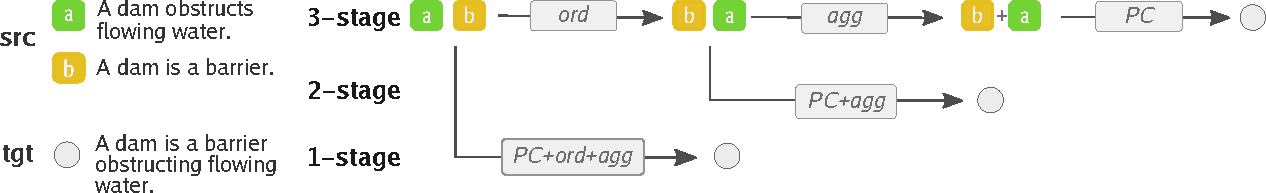
\includegraphics[width=\textwidth]{img/pipeline-variants.pdf}

    \caption{An example illustrating how the individual modules are trained and subsequently applied as the parts of the pipeline. See \autoref{sec:pipeline:implementation} for the description of the ordering model (\textsc{ord}), the aggregation model (\textsc{agg}), and the variants of the paragraph compression model (\textsc{PC, PC+agg, PC+ord+agg}).}
    \label{fig:pipeline:variants}
\end{figure*}


\paragraph{Pipeline versions} To evaluate individual components of our pipeline, we train three versions of the \textit{paragraph compression} model (see \autoref{fig:pipeline:variants}). The models share the same architecture and targets but differ in their inputs:
\begin{itemize}
    \item \textsc{\ac{pc}} -- the model takes as an input ordered facts with delimiters (as described in \autoref{sec:pipeline:method}),
    \item \textsc{\ac{pc}+agg} -- the model takes as an input the ordered facts \textit{without} delimiters (i.e., the aggregation is left implicitly to the model),
    \item \textsc{\ac{pc}+ord+agg} -- the model takes as an input the facts in \textit{random} order and \textit{without} delimiters (i.e., both ordering and aggregation are left implicitly to the model).
\end{itemize}
Correspondingly, we test three versions of the pipeline for the ablation study:
\begin{itemize}
    \item \textsc{3-stage} -- a full version of the pipeline consisting of the ordering model (\textsc{ord}), the aggregation model (\textsc{agg}), and the \textsc{\ac{pc}} model,
    \item \textsc{2-stage} -- a pipeline consisting of the \textsc{ord} model and the \textsc{\ac{pc}+agg} model,
    \item \textsc{1-stage} -- a single stage consisting of the \textsc{\ac{pc}+ord+agg} model.
\end{itemize}
% We evaluate all versions of the pipeline with PC models trained on the \textit{full} and \textit{filtered} versions of the \textsc{WikiFluent} dataset (see §\ref{sec:pipeline:wikifluent}).


\subsection{Evaluation}
\label{sec:pipeline:eval}
We evaluate outputs from the \textsc{\{1,2,3\}-stage} variants of our pipeline using automatic metrics, and we perform a detailed manual error analysis of the model outputs. We also evaluate the performance of the content planning modules and the ability of the PC module to follow the content plan. Finally, we include an intrinsic evaluation of our modules on the \textsc{WikiFluent} test set.

\begin{table*}[t]\centering\footnotesize
    \begin{tabular}{l p{12.2cm}} \toprule
        \textbf{Input}  & \textit{(Allen Forrest; background; solo singer), (Allen Forrest; genre; Pop music), (Allen Forrest; birthPlace; Dothan, Alabama)} \\
        \textbf{Templ.} & Allen Forrest is a solo singer. Allen Forrest performs Pop music. Allen Forrest was born in Dothan, Alabama.                       \\
        \textbf{Model}  & \lightblue{Allen Forrest is a solo singer who performs Pop music. He was born in Dothan, Alabama.}                                 \\
        \textbf{Human}  & Born in Dothan, Alabama, Allen Forrest has a background as a solo singer and was a pop artist.                                     \\\cdashlinelr{1-2}
        \textbf{Input}  & \textit{name[Wildwood], eatType[restaurant], food[French], area[riverside], near[Raja Indian Cuisine]}                             \\
        \textbf{Templ.} & Wildwood is a restaurant. Wildwood serves French food. Wildwood is in the riverside. Wildwood is near Raja Indian Cuisine.         \\
        \textbf{Model}  & \lightblue{Wildwood is a restaurant serving French food. It is in the riverside near Raja Indian Cuisine.}                         \\
        \textbf{Human}  & A amazing French restaurant is called the Wildwood. The restaurant is near the Raja Indian Cuisine in riverside. They love kids.   \\ \bottomrule
    \end{tabular}
    \caption{Example outputs of our model (\textsc{3-stage}, filtered). For each example, we show the input triples, the intermediate templates, the output from the model, and the corresponding human reference.}
    \label{tab:pipeline:ex1}
\end{table*}

\paragraph{Automatic Metrics}


\begin{table}[t]

    \centering \small
    \begin{tabular}{llcccccccc} \toprule
                                                                                       &                  & \multicolumn{4}{c}{\textbf{WebNLG}} & \multicolumn{4}{c}{\textbf{E2E}}                                                                                                       \\
                                                                                       &                  & \textbf{B}                          & \textbf{M}                       & \textbf{O}     & \textbf{H}     & \textbf{B}     & \textbf{M}     & \textbf{O}     & \textbf{H}     \\\midrule
        \multicolumn{2}{l}{\baselinecopy{}}                                            & 37.18            & 38.77                               & 0.000                            & 0.000          & 24.19          & 34.89          & 0.000          & 0.000                           \\\cdashlinelr{1-10}
        \multicolumn{2}{l}{$\text{UPF-FORGe}^*$}                                       & 38.65            & 39.00                               & 0.075                            & 0.101          & -              & -              & -              & -                               \\
        \multicolumn{2}{l}{$\textsc{Melbourne}^*$}                                     & 45.13            & 37.00                               & 0.237                            & 0.202          & -              & -              & -              & -                               \\
        \multicolumn{2}{l}{$\text{\citet{keJointGTGraphTextJoint2021}}^{\dagger *}$}   & 66.14            & 47.25                               & -                                & -              & -              & -              & -              & -                               \\
        \multicolumn{2}{l}{$\text{\citet{laha2020scalable}}^{\dagger}$}                & 24.80            & 34.90                               & -                                & -              & -              & -              & -              & -                               \\\cdashlinelr{1-10}
        \multicolumn{2}{l}{\textsc{TGen}$^*$}                                          & -                & -                                   & -                                & -              & 40.73          & 37.76          & 0.016          & 0.083                           \\
        \multicolumn{2}{l}{\citet{harkousHaveYourText2020}$^{\dagger *}$}\hspace{-2mm} & -                & -                                   & -                                & -              & 43.60          & 39.00          & -              & -                               \\\midrule
        \multirow{3}{*}{\textit{full}}                                                 & \textsc{3-stage} & 42.92                               & 39.07                            & 0.051          & 0.148          & \textbf{36.04} & 36.95          & \textbf{0.001} & \textbf{0.001} \\
                                                                                       & \textsc{2-stage} & 42.90                               & 39.28                            & \textbf{0.043} & 0.125          & 35.84          & 36.91          & \textbf{0.001} & \textbf{0.001} \\
                                                                                       & \textsc{1-stage} & 39.08                               & 38.94                            & 0.071          & 0.204          & 30.81          & 36.01          & 0.009          & 0.122          \\\cdashlinelr{1-10}
        \multirow{3}{*}{\textit{filtered}}                                             & \textsc{3-stage} & 43.19                               & 39.13                            & 0.152          & \textbf{0.073} & 35.88          & 36.95          & \textbf{0.001} & \textbf{0.001} \\
                                                                                       & \textsc{2-stage} & \textbf{43.49}                      & \textbf{39.32}                   & 0.146          & 0.096          & 36.01          & \textbf{36.99} & \textbf{0.001} & \textbf{0.001} \\
                                                                                       & \textsc{1-stage} & 42.99                               & 38.81                            & 0.202          & 0.093          & 34.08          & 36.32          & 0.012          & 0.050          \\ \bottomrule
    \end{tabular}
    \caption{Automatic metrics on the WebNLG and E2E datasets. B = BLEU, M = METEOR, O = omissions / \# facts, H = hallucinations / \# examples. The systems marked with asterisk (*) are trained on the in-domain data. The results for the systems marked with $\dagger$ are taken from the respective works. \textbf{Boldface} denotes the best variant of our zero-shot system.}
    \label{tab:pipeline:auto}
\end{table}



Following prior work, we use BLEU \cite{papineni2002bleu} and METEOR \cite{banerjee-lavie-2005-meteor} to evaluate the outputs against the human references.\footnote{We use the implementation from \url{https://github.com/tuetschek/e2e-metrics}.} We also evaluate the number of omission and hallucination errors (i.e., facts missing or added, respectively) using a metric from \citet{dusekEvaluatingSemanticAccuracy2020} based on a RoBERTa model \cite{liuRoBERTaRobustlyOptimized2019} pretrained on natural language inference (see \autoref{sec:sem-acc}.

We include a diverse set of baselines for comparison. \baselinecopy{} denotes the baseline of copying the facts without further processing. For WebNLG, we further compare our systems with the results of:
\begin{itemize}
    \item UPF-FORGe and \textsc{Melbourne} -- systems (grammar-based and supervised, respectively) from the first run of WebNLG Challenge \cite{gardentWebNLGChallengeGenerating2017},
    \item  \citet{keJointGTGraphTextJoint2021} -- a state-of-the-art system with a structure-aware encoder and task-specific pretraining,
    \item \citet{laha2020scalable} -- a zero-shot D2T generation system.
\end{itemize}
For E2E, we compare our systems with the results of:
\begin{itemize}
    \item \textsc{TGen} \cite{dusekTrainingNaturalLanguage2015} -- the baseline system for the E2E Challenge \cite{dusekEvaluatingStateoftheartEndtoEnd2020},
    \item \citet{harkousHaveYourText2020} -- a state-of-the-art supervised system on the cleaned version of E2E data.
\end{itemize}

The automatic evaluation (\autoref{tab:pipeline:auto}) shows that our systems consistently outperform the \baselinecopy{} baseline (e.g., $\sim$12 BLEU points for E2E), which is already strong thanks to our manually curated set of templates.\footnote{On WebNLG, \baselinecopy{} achieves 37.18 BLEU points, compared to 24.80 BLEU points of the \textit{full system} of \citet{laha2020scalable}, which uses automatic template generation.} Automatic scores also suggest that our systems are comparable with some older supervised systems, although they underperform the state-of-the-art supervised systems.

The \textsc{2-stage} system is generally on par with the \textsc{3-stage} system, which indicates that explicit aggregation using the \textsc{agg} model may not be necessary. However, a separate aggregation module allows one to control the aggregation step explicitly. The models using the filtered version of the corpus generally produce better results, although they also bring in a larger number of omissions.


\paragraph{Manual Error Analysis}

\begin{table}[t]
    \centering\small
    \begin{tabular}{l l ccccc >{\hspace{3mm}}ccccc} \toprule
         &                  & \multicolumn{5}{c}{\bf WebNLG} & \multicolumn{5}{c}{\bf E2E}                                                                                                         \\
         &                  & \textbf{H}                     & \textbf{I}                  & \textbf{O} & \textbf{R} & \textbf{G} & \textbf{H} & \textbf{I} & \textbf{O} & \textbf{R} & \textbf{G} \\\midrule
        \multirow{3}{*}{\textit{full}}
         & \textsc{3-stage} & 3                              & 39                          & 2          & 2          & 16         & 0          & 1          & 0          & 0          & 17         \\
         & \textsc{2-stage} & 8                              & 36                          & 1          & 5          & 16         & 1          & 1          & 0          & 1          & 23         \\
         & \textsc{1-stage} & 28                             & 27                          & 6          & 10         & 20         & 17         & 0          & 1          & 79         & 45         \\\cdashlinelr{1-12}
        \multirow{3}{*}{\textit{filtered}}
         & \textsc{3-stage} & 2                              & 37                          & 2          & 1          & 15         & 0          & 0          & 0          & 0          & 17         \\
         & \textsc{2-stage} & 5                              & 32                          & 1          & 2          & 14         & 0          & 0          & 0          & 0          & 11         \\
         & \textsc{1-stage} & 8                              & 40                          & 6          & 6          & 16         & 11         & 2          & 1          & 41         & 22         \\\bottomrule
    \end{tabular}
    \caption{Number of manually annotated errors on 100 examples: H = hallucinations, I = incorrect fact merging, O = omissions, R = redundancies, G = grammar errors or disfluencies.}
    \label{tab:pipeline:manual}
\end{table}
We manually examined 100 model outputs, counting the number of factual (hallucinations, omissions, incorrect fact merging, redundancies) and grammatical errors. The results are summarized in Table \ref{tab:pipeline:manual}.

The \textsc{1-stage} model (which has to order the facts implicitly) tends to repeat the facts in the text (especially in E2E) and produces frequent hallucinations. These problems are largely eliminated with the \textsc{2-stage} and \textsc{3-stage} models, which produce almost no hallucinations or omissions.

However, the outputs on WebNLG for all systems suffer from semantic errors resulting from merging unrelated facts. This mostly happens with unrelated predicates connected to the same subject/object (e.g., ``X was born in Y'', ``X worked as Z'' expressed as ``X worked as Z in Y''). On the E2E data, where predicates share the same subject, the outputs are generally consistent, and the \textsc{2-stage} and \textsc{3-stage} models exhibit almost no semantic errors. Grammar errors and disfluencies stem mainly from over-eager paragraph compression or from artifacts in our templates and are relatively minor (e.g., missing ``is'' in ``serves French food and family-friendly'').


\paragraph{Content Planning} We manually evaluate how the \ac{pc} model follows the content plan (i.e., keeping the predefined order and aggregating the sentences according to the delimiters) using 100 randomly chosen examples with more than one triple on WebNLG and E2E. We find that the model follows the content plan in 95\% and 100\% of cases, respectively. The incorrect cases include mainly a fact not properly mentioned or an extra boundary between sentences without a separator. We can thus conclude that the pretraining task successfully teaches the PC model to follow a given content plan.


% Following \citet{su2021plan} and \citet{zhao2020bridging}, we report the accuracy and BLEU-2 score of our \textbf{ordering model} on WebNLG against the human-generated plans from \citet{ferreira2018enriching}. The results are listed in Table \ref{tab:cp} and compared against a \textsc{random} baseline (random ordering) and prior work. The results show that although our approach again lags behind state-of-the-art supervised approaches, it can outperform both the random baseline and the Transformer-based approach from \citet{ferreira2019neural} while not using any in-domain examples.

% \begin{table}[t]
%     \centering\small
%     \begin{tabular}{lcc} \toprule
%                                                         & \textbf{B-2} & \textbf{Acc} \\ \midrule
%         Transformer \cite{ferreira2019neural}$^\dagger$ & 52.20        & 0.35         \\
%         Step-by-step \cite{moryossef2019step}$^\dagger$ & 70.80        & 0.47         \\
%         PLANENC \cite{zhao2020bridging}$^\dagger$       & 80.10        & 0.62         \\
%         Plan-then-generate \cite{su2021plan}$^\dagger$  & 84.97        & 0.72         \\\cdashlinelr{1-3}
%         \textsc{random}                                 & 47.00        & 0.29         \\ \midrule
%         Ours (BART+ptr)                                 & 59.10        & 0.48         \\ \bottomrule
%     \end{tabular}
%     \caption{Evaluation of our zero-shot ordering model based on \citet{calizzano2021ordering}. B-2 = BLEU-2, Acc = accuracy. The results marked with $\dagger$ are copied from the respective papers.}
%     \label{tab:pipeline:cp}
% \end{table}

% We also evaluate the accuracy of our \textbf{aggregation model}, using triples ordered according to the plans from \citet{ferreira2018enriching} as input. The accuracy is 0.33 per example and 0.62 per sentence boundary (random baseline is 0.23 and 0.50, respectively). The results show that although our approach is better than the random baseline, there is still room for improvement.

% Finally, 

% \paragraph{Intrinsic Evaluation} We also provide evaluation of our pipeline modules on the \mbox{\textsc{WikiFluent}} test sets. We evaluated the ordering, aggregation, and paragraph compression modules trained on the \textit{full} \textsc{WikiFluent} corpus. The results for both \textit{full} and \textit{filtered} test sets are summarized in Table \ref{tab:wikifluent_test}. The PC model achieves high scores, which follows from the fact that we provide it with ground truth content plans (i.e., the ordering and aggregation plan corresponding to the original paragraph). Accuracy of the ordering and aggregation modules is comparable to their performance on D2T datasets.

% \begin{table}[t]
%     \centering\small
%     \begin{tabular}{ll cc} \toprule
%                                           &                       & \textbf{test (full)} & \textbf{test (filt.)} \\\midrule
%         \multirow{2}{*}{\textsc{ord}}     & BLEU-2                & 64.8                 & 71.9                  \\
%                                           & Accuracy              & 0.70                 & 0.77                  \\ \midrule
%         \multirow{2}{*}{\textsc{Agg}}     & Acc. per example      & 0.68                 & 0.68                  \\
%                                           & Acc. per sent. bound. & 0.93                 & 0.93                  \\ \midrule
%         \multirow{2}{*}{\textsc{\ac{pc}}} & BLEU                  & 90.72                & 91.60                 \\
%                                           & METEOR                & 63.89                & 65.03                 \\ \bottomrule
%     \end{tabular}
%     \caption{Result of individual pipeline modules on the \textsc{WikiFluent} test sets (full / filtered). The metrics correspond to the metrics used for evaluating the modules for D2T generation.}
%     \label{tab:wikifluent_test}
% \end{table}
